\documentclass{llncs}
%
%
%espero que no se enfaden por incluir este paquete:
\usepackage{amsmath}
\usepackage{amssymb}
%\usepackage{amsthm}

\usepackage[dvips]{graphicx}
\usepackage{makeidx}  % allows for indexgeneration
\usepackage{color}
\usepackage[table]{xcolor}
\usepackage{caption}
\usepackage{subcaption}
\usepackage{algorithm2e}
\usepackage{multirow}

\hyphenation{pro-per-ties}
\hyphenation{ge-ne-ral-ly}
\hyphenation{pre-fe-ren-ces}
\hyphenation{u-sing}
\hyphenation{pu-nish-ment}
\newcommand{\Pow}{\mathcal{P}}
\newcommand{\N}{\operatorname{N}}
\newcommand{\bool}{\operatorname*{\mathcal{B}}}
\newcommand{\Pos}{\operatorname{Pos}}
\newcommand{\Nec}{\operatorname{Nec}}
\newcommand{\Open}{\operatorname{Open}}
\newcommand{\Rp}{\operatorname{Rp}}
\newcommand{\Rn}{\operatorname{Rn}}
\newcommand{\FB}{\operatorname{FB}}
\newcommand{\UC}{\operatorname{UC}}
\newcommand{\T}{\mathcal{T}}
\newcommand{\Rel}{\mathcal{R}}
\newcommand{\C}{\mathcal{C}}
\newcommand{\Nat}{\mathbb{N}}
\newcommand{\Boolean}{\mathbb{B}}
\newcommand{\Q}{\mathbb{Q}}
\newcommand{\R}{\mathbb{R}}
\newcommand{\Z}{\mathbb{Z}}
\newcommand{\Head}{\mathcal{H}}
\newcommand{\Body}{\mathcal{B}}
\newcommand{\Dom}{\mathcal{D}}
\newcommand{\INS}{\mbox{\textbf{insert}}}
\newcommand{\DEL}{\mbox{\textbf{delete}}}
\newcommand{\MOD}{\mbox{\textbf{modify}}}
\newcommand{\REV}{\mbox{\textbf{revise}}}
\newcommand{\Overlap}{\mbox{\textbf{Overlap}}}
\newcommand{\A}{\mathcal{A}}
\newcommand{\I}{\mathcal{I}}
\renewcommand{\Join}{\bowtie}



\usepackage[textwidth=2.2cm]{todonotes}
%\usepackage[disable]{todonotes}

%\theoremstyle{definition}
%\newtheorem{definition}{Definition}
\begin{document}

\mainmatter              % start of the contributions
%
\title{Evaluation of the Allen's relations for two Possibilistic Time Periods.}
%
%\titlerunning{A Fuzzy Valid-Time Model}  % abbreviated title (for running head)
%                                     also used for the TOC unless
%                                     \toctitle is used
%
\author{
%Jos\'e Enrique Pons
 }
%Jeffrey Dean \and David Grove \and Craig Chambers \and Kim~B.~Bruce \and
%Elsa Bertino}
%
\authorrunning{Jos\'e Enrique Pons et al.} % abbreviated author list (for running head)
%
%%%% list of authors for the TOC (use if author list has to be modified)
%\tocauthor{Ivar Ekeland, Roger Temam, Jeffrey Dean, David Grove,
%Craig Chambers, Kim B. Bruce, and Elisa Bertino}
%
\institute{
% Department of Computer Science and Artificial Intelligence \\
% Universidad de Granada \\
% Escuela T\'ecnica Superior de Ingenier\'ia Inform\'atica \\
% C/Periodista Daniel Saucedo Aranda s/n \\
% E-18071 (Granada-Spain)\\
% \email{jpons,opc@decsai.ugr.es}\\ 
%WWW home page:
%\texttt{http://users/\homedir iekeland/web/welcome.html}
%\and
%Universit\'{e} de Paris-Sud,
%Laboratoire d'Analyse Num\'{e}rique, B\^{a}timent 425,\\
%F-91405 Orsay Cedex, France
}

\maketitle              % typeset the title of the contribution

\begin{abstract}

\end{abstract}

\section{\label{sec:intro}Introduction}
In this work we propose the evaluation of the Allen's relations for time intervals for two given possibilistic time periods.


\section{\label{sec:implementation}Implementation of the Allen's Relations}

In the following we will consider a possibilistic time interval (\emph{PTI}) be $I = \left[S_i, E_i \right]$. Where $S_i$ and $E_i$ are possibilistic time points representing the starting and the ending boundaries of the time interval.

Each possibilistic time point is given by $P = \left[D, a, b \right]$. This notation represents that:
\begin{itemize}
 \item $D$ is the central main point.
\item $D-a$ is the left point.
\item $D+b$ is the right point.
\end{itemize}
 
In the following, a time interval $I$ will be noted as:
\begin{align}
 I = \left[S_i, E_i \right]\\
S_i = \left[D_{S_i},a_{S_i},b_{S_i} \right] \\
E_i = \left[D_{E_i},a_{E_i},b_{E_i} \right]
\end{align}

% The following proposal translates an interval end-points constraint to several ill-known constraints that allows the evaluation for two pvps.

A relation between two crisp time points $m, n$ is given by the following expression.
\begin{equation}
\label{eq:general-crisp-comparison}
\left(n\  R \  m \right) 
\end{equation}
Where  $R$ is one of the following: $\left \lbrace <, >, \leq, \geq, = \right \rbrace$.
The result of the expression is a boolean value indicating whether the point $n$ is in the relation $\left( R, m \right)$.

\begin{equation}
\label{eq:boolean-crisp-comparison}
n \in A:\left(a, m \right) \in R
\end{equation}

% A crisp constraint can be translated to a set of two ill-known constraint. First of all, the end-points $a, b$ are in the possibilistic case to two ill-known time points: $A_i, B_j$
% \begin{equation}
%  \left( =, A_i \right) \wedge \left(R, B_j \right)
% \end{equation}
\subsection{\label{subsec:translation}Translation to the possibilistic case}
In order to implement the Allen's relations for two possibilistic valid-time periods, we need to translate the expression in \eqref{eq:general-crisp-comparison} to the possibilistic case. In this case, we will note \eqref{eq:general-crisp-comparison} as the following:

\begin{equation}
\label{eq:general-possibilistic-comparison}
\left(P_n\  R \  P_m \right) 
\end{equation}

Where:
\begin{itemize}
 \item  $P_n$ is either the starting or ending point of the possibilistic time interval given by $I = \left[S_i, E_i \right]$.
\item $P_m$ is either the starting or ending point of the possibilistic time interval given by $J = \left[S_j, E_j \right]$.
\item $R \in \left \lbrace <, >, \leq, \geq, = \right \rbrace$.
\end{itemize}

The evaluation of the expression \eqref{eq:general-possibilistic-comparison} is equivalent to the following ill-known constraints:
\begin{align}
 \label{eq:evaluation-by-ill-known}
\left(P_n\  R \  P_m \right)  &\triangleq \lambda \left( C_1 , C_2 \right) \\
\nonumber
& C_1 =\left(=, P_n \right) \\
\nonumber
& C_2 = \left(R, P_m \right)
\end{align}

Consider that $a \in A \subseteq U$, then:
\begin{align}
 \label{eq:evaluation-1}
\Pos \left(C_1 \left(A \right)\right) &= \min_{a  \in A} \left(\pi_{P_n} \left(a \right) \right)\\
\nonumber
\Nec \left(C_1 \left(A \right) \right) &= \min_{a  \in A} \left(1-\pi_{P_n} \left(a \right)\right)\\
\nonumber
\Pos \left(C_2 \left(A \right)\right) &= \min_{a \in A} \left(\sup_{\left \lbrace a , \omega \right \rbrace \in R}  \pi_{P_m} \left(\omega \right) \right)\\
\nonumber
\Nec \left(C_2 \left(A \right) \right) &= \min_{a \in A} \left(\inf_{\left \lbrace a, \omega \right \rbrace  \not \in R} 1-\pi_{P_m}\left(\omega \right) \right)
\end{align}

With $\lambda = \left(\wedge, \left(C_1, C_2 \right) \right)$, we obtain:
\begin{align}
 \label{eq:eval-2}
\Pos \left(\lambda \left(A \right)\right) &= \max \min_{a \in A} \left(\Pos \left(C_1 \left( A\right) \right), \Pos \left(C_2\left(A \right) \right) \right)\\
\nonumber
\Nec \left(\lambda \left(A\right)\right) &= \max \min_{a \in A} \left(\Nec \left(C_1 \left( A\right) \right), \Nec \left(C_2\left(A \right) \right) \right)
\end{align}






\subsection{\label{subsec:before}Before}
The crisp version for the before operator for two crisp intervals $i = \left[s_i,e_i \right], j = \left[s_j, e_j \right]$.
\begin{equation}
i \mbox{ Before } j \triangleq \left( e_i < s_j \right)
\end{equation}
This is translated to the possibilistic case:
$I = \left[S_i, E_i \right], J = \left[S_j, E_j\right]$.

\begin{align}
 I \mbox{ Before } J &\triangleq \lambda \left(C_1, C_2 \right)\\
\nonumber
C_1 &\triangleq \left(=, E_i\right) \\
\nonumber
C_2 &\triangleq \left(<, S_j \right)
\end{align}
The possibility and the necessity of the Before relation is computed as follows:
\begin{align}
\Pos \left(\lambda \left(A \right)\right) &= \max \min_{a \in A} \left(\Pos \left(C_1 \left( A\right) \right), \Pos \left(C_2\left(A \right) \right) \right)\\
\nonumber
\Nec \left(\lambda \left(A\right)\right) &= \min \min_{a \in A} \left(\Nec \left(C_1 \left( A\right) \right), \Nec \left(C_2\left(A \right) \right) \right)
\end{align}




\begin{example}
Consider the following possibilistic time periods:
\begin{align}
I = \left( \left[1,2,2 \right] , \left[6,2,2 \right] \right)\\
\nonumber
J = \left( \left[6,1,1 \right] , \left[9,1,1 \right] \right)
\end{align}

We want to know the possibility of $I$ Before $J$. As a result of triangle's line intersection, we get:
\begin{align}
 \label{sample:before}
\Pos \left(\lambda \left(A \right)\right) &= - \frac{-D_{S_j} + D_{E_i}-a_{E_i}}{a_{S_j}+a_{E_i}}\\
\nonumber
&= - \frac{-6+6-2}{2+1} = \frac{2}{3}\\
\Nec \left(\lambda \left(A\right)\right) &= 0
\end{align}


\begin{figure}[ht]
\caption{Illustration of the before relationship.}
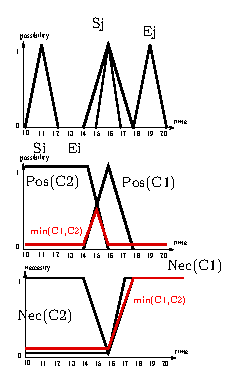
\includegraphics[scale=2.1]{./graphs/before.eps} 
\end{figure}



\end{example}





\section{\label{sec:evaluation}Evaluation }
In this section we will explain the evaluation of the Allen's relations in the possibilistic case defined by sets of ill-known constraints.
First of all, we will consider that the representation for both starting and ending points is a triangular membership function. Therefore, the possibilistic interval is defined by two triangular membership functions.
The membership function for a time point $X = \left[D, a, b \right]$ is given by the following equation:

\begin{equation}
 \label{eq:triangular-membership}
\mu\left(x \right) =
\begin{cases}
 0, & \mbox{ if } x \leq \left(D-a \right) \vee x \geq \left( D+b\right)\\
1, & \mbox{ if } x = D\\
\frac{x-(D-a)}{a} , & \mbox{ if } x > \left(D-a \right) \wedge x< D\\
\frac{D+b-x}{b} , & \mbox{ if } x > D \wedge x< \left(D +b\right)
\end{cases}
\end{equation}

The last two cases are based on the equation for the line and a point. The following equations are the membership functions for the ill-known constraints:

\begin{itemize}
 \item $\left(<, X \right)$:
	\begin{equation}
	 \label{eq:ikc-lt}
	  \mu\left(x \right) =
	      \begin{cases}
			  1, & \mbox{ if } x \leq D-a\\
			  0, & \mbox{ if } x \geq D\\
			  \frac{x-D}{a} , & \mbox{ if } x > \left(D-a \right) \wedge x< D\\			  
			  \end{cases}
	\end{equation}
\item $\left(\leq, X \right)$
	\begin{equation}
		\label{eq:ikc-leq}
		  \mu\left(x \right) =
		      \begin{cases}
				  1, & \mbox{ if } x \leq D\\
				  0, & \mbox{ if } x \geq D+b\\
				  \frac{D+b-x}{b} , & \mbox{ if } x > D \wedge x< \left(D+b\right)\\			  
				  \end{cases}
		\end{equation}
\item $\left(>, X \right)$
	\begin{equation}
		\label{eq:ikc-gt}
		  \mu\left(x \right) =
		      \begin{cases}
				  0, & \mbox{ if } x \leq D\\
				  1, & \mbox{ if } x \geq D+b\\
				  \frac{x-D}{b} , & \mbox{ if } x > D \wedge x< \left(D+b\right)\\			  
				  \end{cases}
		\end{equation}

\item $\left(\geq, X \right)$
	\begin{equation}
		\label{eq:ikc-geq}
		  \mu\left(x \right) =
		      \begin{cases}
				  0, & \mbox{ if } x \leq \left(D-a \right)\\
				  1, & \mbox{ if } x \geq D\\
				  \frac{x-\left(D-a\right)}{a} , & \mbox{ if } x > \left(D-a\right) \wedge x< D\\			  
				  \end{cases}
		\end{equation}
\item $\left(=, X \right)$, see equation \eqref{eq:triangular-membership}.

\item $\left(\neq, X \right)$
	\begin{equation}
		\label{eq:ikc-neq}
		  \mu\left(x \right) =
		      \begin{cases}
				  1, & \mbox{ if } x \leq \left(D-a\right) \wedge x \geq \left(D+b \right)\\
				  \frac{D-x}{a} , & \mbox{ if } x > \left(D-a\right) \wedge x< D\\
				  \frac{x-D}{b} , & \mbox{ if } x > D \wedge x< \left(D+b \right)\\	
				  \end{cases}
		\end{equation}

	
\end{itemize}




\begin{figure} 
\centering
\begin{subfigure}[b]{0.3\textwidth}
  \centering
  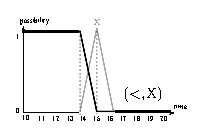
\includegraphics[width=\textwidth]{graphs/lt.eps}
%   \caption{See equation \eqref{eq:ikc-lt}}
%   \label{fig:lt}
\end{subfigure}
~
\begin{subfigure}[b]{0.3\textwidth}
  \centering
  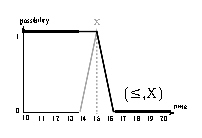
\includegraphics[width=\textwidth]{graphs/lte.eps}
%   \caption{See equation \eqref{eq:ikc-leq}}
%   \label{fig:lte}
\end{subfigure}

\begin{subfigure}[b]{0.3\textwidth}
  \centering
  
\includegraphics[width=\textwidth]{graphs/gt.eps}
%   \caption{See equation \eqref{eq:ikc-gt}}
%   \label{fig:gt}
\end{subfigure}
~
\begin{subfigure}[b]{0.3\textwidth}
  \centering
  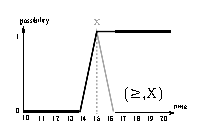
\includegraphics[width=\textwidth]{graphs/gte.eps}
%   \caption{See equation \eqref{eq:ikc-gte}}
%   \label{fig:gte}
\end{subfigure}

\begin{subfigure}[b]{0.3\textwidth}
  \centering
  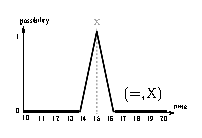
\includegraphics[width=\textwidth]{graphs/eq.eps}
%   \caption{See equation \eqref{eq:triangular-membership}}
%   \label{fig:eq}
\end{subfigure}
~
\begin{subfigure}[b]{0.3\textwidth}
  \centering
  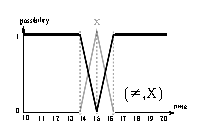
\includegraphics[width=\textwidth]{graphs/neq.eps}
%   \caption{See equation \eqref{eq:ikc-neq}}
%   \label{fig:neq}
\end{subfigure}
\caption{Representation for the membership functions for each ill-known constraint.}
\end{figure}




The algorithm to compute the intersections between two ill-known constraints is given by the following algorithm:
\begin{algorithm}
\SetLine
\linesnumbered
\SetKwInOut{Input}{input}
\SetKwInOut{Output}{output}


\Input{Two ill-known values $X, Y$ with triangular membership functions and two ill-known constraints in the form $C_1 \triangleq \left(\theta, Y \right)$, $C_2 \triangleq \left(=, X \right)$}
\Output{The possibility degree for $C_1 \wedge C_2$}
\caption{Computation of the possibility for two ill-known constraints.}
 \KwData{\;
$X=\left[D_x, a_x, b_x \right]$\;
$Y=\left[D_y, a_y, b_y \right]$\;
$C_1 \triangleq \left( \theta, Y \right), \theta \in \left(<,\leq,> ,\geq \right)$\;
$C_2 \triangleq \left( =, X \right)$
}
\KwResult{$\Pos \left(C_1 \wedge C_2 \right)$}
\BlankLine
\tcc{Based on the standard equation of a line passing through 2 points:}
gen:$\gets \frac{x-x_1}{x_2-x_1} = \frac{y-y_1}{y_2-y_1}$\;
\tcc{The definition of the left and the right lines for the ill-known constraint $\left(=, X \right)$:}
li:$\leftarrow$gen $\left \lbrace x_1 = \left(D_x-a_x\right), x_2 = D_x, y_1 = 0, y_2 = 1 \right \rbrace$\;
ld:$\leftarrow$gen $\left \lbrace x_1 = \left(D_x+b_x\right), x_2 = D_x, y_1 = 0, y_2 = 1 \right \rbrace$\;

$sol\gets \emptyset$ \tcc*[l]{The set that contains the candidate solutions}
\Switch{$\theta$}
{
\Case{$<$}{
ld1:$\leftarrow$gen $\left \lbrace x_1 = \left(D_y+a_y\right), x_2 = D_y, y_1 = 1, y_2 = 0 \right \rbrace$\;
% $sol_1 \leftarrow $ solve (li,ld1 ) = $sol_1 = -\frac{-D_y+D_x-a_x}{a_x+a_y}$\;
% $sol_2 \leftarrow $ solve (ld,ld1 ) = $sol_2 = \frac{-D_y+D_x+b_x}{b_x+a_y}$\;
}
\Case{$\leq$}{
ld1:$\leftarrow$gen $\left \lbrace x_1 = \left(D_y+b_y\right), x_2 = D_y, y_1 = 0, y_2 = 1 \right \rbrace$\;
% $sol_1 \leftarrow $ solve (li,ld1 ) = $sol_1 = -\frac{-D_y+D_x-b_y-a_x}{a_x+b_y}$\;
% $sol_2 \leftarrow $ solve (ld,ld1 ) = $sol_2 = \frac{-D_y+D_x-b_y+b_x}{b_x-b_y}$\;
}
\Case{$>$}{
li1:$\leftarrow$gen $\left \lbrace x_1 = D_y, x_2 = \left(D_y+b_y \right), y_1 = 0, y_2 = 1 \right \rbrace$\;
% $sol_1 \leftarrow $ solve (li,li1 ) = $sol_1 = -\frac{-D_y+D_x-a_x}{a_x-b_y}$\;
% $sol_2 \leftarrow $ solve (ld,li1 ) = $sol_2 = \frac{-D_y+D_x+b_x}{b_x+b_y}$\;
}
\Case{$\geq$}{
li1:$\leftarrow$gen $\left \lbrace x_1 = D_y, x_2 = \left(D_y-a_y \right), y_1 = 1, y_2 = 0 \right \rbrace$\;
% $sol_1 \leftarrow $ solve (li,li1 ) = $sol_1 = -\frac{-D_y+D_x+a_y-a_x}{a_x-a_y}$\;
% $sol_2 \leftarrow $ solve (ld,li1 ) = $sol_2 = \frac{-D_y+D_x+b_x+a_y}{b_x+a_y}$\;
}
\Case{$=$}{
ld1:$\leftarrow$gen $\left \lbrace x_1 = \left(D_y+b_y\right), x_2 = D_y, y_1 = 0, y_2 = 1 \right \rbrace$\;
li1:$\leftarrow$gen $\left \lbrace x_1 = D_y, x_2 = \left(D_y-a_y \right), y_1 = 1, y_2 = 0 \right \rbrace$\;
% $sol_1 \leftarrow $ solve (li,ld1 ) = $sol_1 = -\frac{-D_y+D_x-a_x}{a_x+a_y}$\;
% $sol_2 \leftarrow $ solve (ld,ld1 ) = $sol_2 = \frac{-D_y+D_x+b_x}{b_x+a_y}$\;
% $sol_3 \leftarrow $ solve (li,li1 ) = $sol_3 = -\frac{-D_y+D_x+a_y-a_x}{a_x-a_y}$\;
% $sol_4 \leftarrow $ solve (ld,li1 ) = $sol_4 = \frac{-D_y+D_x+b_x+a_y}{b_x+a_y}$\;

}
\Case{$\neq$}{
ld1:$\leftarrow$gen $\left \lbrace x_1 = \left(D_y+a_y\right), x_2 = D_y, y_1 = 1, y_2 = 0 \right \rbrace$\;
li1:$\leftarrow$gen $\left \lbrace x_1 = D_y, x_2 = \left(D_y+b_y \right), y_1 = 0, y_2 = 1 \right \rbrace$\;
% $sol_1 \leftarrow $ solve (li,ld1 ) = $sol_1 = -\frac{-D_y+D_x-b_y-a_x}{a_x+b_y}$\;
% $sol_2 \leftarrow $ solve (ld,ld1 ) = $sol_2 = \frac{-D_y+D_x-b_y+b_x}{b_x-b_y}$\;
% $sol_3 \leftarrow $ solve (li,li1 ) = $sol_3 = -\frac{-D_y+D_x-a_x}{a_x-b_y}$\;
% $sol_4 \leftarrow $ solve (ld,li1 ) = $sol_4 = \frac{-D_y+D_x+b_x}{b_x+b_y}$\;
}
}
\tcc{Now compute the intersections between each pair of lines:}
$sol_1 \leftarrow $ solve (li,ld1 )\;
$sol_2 \leftarrow $ solve (ld,ld1 )\;
$sol_3 \leftarrow $ solve (li,li1 )\;
$sol_4 \leftarrow $ solve (ld,li1 )\;
\tcc{Finally get the result value:}
$\max \gets 0$\;
\lForEach{$sol[i] \in sol$}
{
\uIf{$sol[i] \in \left[0, 1 \right] \wedge sol[i] > \max$}{ $\max = sol[i]$\;}
}
\KwRet{$\max$\;}
\end{algorithm}

For a quick reference, the following table \ref{tbl:function-solve} presents the results for the function solve(l1,l2).

% \vspace{-10pt}

\begin{table}
\centering
\caption{Results for the function solve}

\begin{tabular}{c l }
\hline
Operator & Results \\ \hline
\multirow{2}{*}{$<$} 
 & $sol_1 = -\left({-D_y+D_x-a_x}\right)/\left({a_x+a_y}\right)$ \\
 & $sol_2 = \left({-D_y+D_x+b_x}\right)/\left({b_x+a_y}\right)$ \\ \hline
\multirow{2}{*}{$\leq$}
 & $sol_1 = -\left({-D_y+D_x-b_y-a_x}\right)/\left({a_x+b_y}\right)$ \\
&  $sol_2 = \left({-D_y+D_x-b_y+b_x}\right)/\left({b_x-b_y}\right)$ \\ \hline
\multirow{2}{*}{$>$}
& $sol_1 = -\left({-D_y+D_x-a_x}\right)/\left({a_x-b_y}\right)$\\
& $sol_2 = \left({-D_y+D_x+b_x}\right)/\left({b_x+b_y}\right)$ \\ \hline
\multirow{2}{*}{$\geq$}
& $sol_1 = -\left({-D_y+D_x+a_y-a_x}\right)/\left({a_x-a_y}\right)$\\
& $sol_2 = \left({-D_y+D_x+b_x+a_y}\right)/\left({b_x+a_y}\right)$ \\
\multirow{4}{*}{$=$}
& $sol_1 = -\left({-D_y+D_x-a_x}\right)/\left({a_x+a_y}\right)$ \\
& $sol_2 = \left({-D_y+D_x+b_x}\right)/\left({b_x+a_y}\right)$ \\
& $sol_3 = -\left({-D_y+D_x+a_y-a_x}\right)/\left({a_x-a_y}\right)$ \\
& $sol_4 = \left({-D_y+D_x+b_x+a_y}\right)/\left({b_x+a_y}\right)$ \\ \hline
\multirow{4}{*}{$\neq$}
& $sol_1 = -\left({-D_y+D_x-b_y-a_x}\right)/\left({a_x+b_y}\right)$ \\
& $sol_2 = \left({-D_y+D_x-b_y+b_x}\right)/\left({b_x-b_y}\right)$ \\
& $sol_3 = -\left({-D_y+D_x-a_x}\right)/\left({a_x-b_y}\right)$ \\
& $sol_4 = \left({-D_y+D_x+b_x}\right)/\left({b_x+b_y}\right)$ \\
\hline 
\end{tabular}
\label{tbl:function-solve}

% \vspace{10pt}


\end{table}

% \vspace{-25pt}





\begin{table}
\centering
\caption{Allen's relations for two ill-known values}

\begin{tabular}{c c c c}
\hline
Relation & Crisp relation & Ill-known constraints & Combination \\ \hline
\multirow{2}{*}{Before}
&  $e_i < s_j$ & $C_1 \triangleq \left(<, S_j \right)$ & $C_1 \wedge C_2$\\
& & $C_2 \triangleq \left(= , E_i \right)$ &\\ \hline
\multirow{4}{*}{Equals}
&  $e_i = e_j \wedge $ & $C_1 \triangleq \left(=, E_i \right)$ & $C_1 \wedge C_2$\\
& $s_i = s_j $& $C_2 \triangleq \left(= , E_j \right)$ & $\wedge$\\
& & $C_3 \triangleq \left(= , S_i \right)$ & $C_3 \wedge C_4$\\
& & $C_4 \triangleq \left(= , S_j \right)$ &\\ \hline
\multirow{5}{*}{Overlaps}
&  $s_i < s_j \wedge $ & $C_1 \triangleq \left(< , S_j \right)$ & $C_1 \wedge C_2$\\
& $e_i > s_j \wedge $  & $C_2 \triangleq \left(= , S_i \right)$ & $\wedge$\\
& $e_i < e_j $         & $C_3 \triangleq \left(> , S_j \right)$ & $C_3 \wedge C_4$\\
&                      & $C_4 \triangleq \left(= , E_i \right)$ & $\wedge $ \\
&                      & $C_5 \triangleq \left(< , E_j \right)$ & $ C_5 \wedge C_4 $\\ \hline
\multirow{2}{*}{Meets}
& $e_i = s_j$ & $C_1 \triangleq \left(= , S_j \right)$ & $C_1 \wedge C_2$\\
&	      & $C_2 \triangleq \left(= , E_i \right)$ & \\ \hline
\multirow{5}{*}{During}
&  $ \left( s_i < s_j \wedge \right. $ & $C_1 \triangleq \left(< , S_j \right)$     & $ \left( C_1 \wedge C_2 \right.$\\
& $\left. e_i \leq e_j\right) \vee $   & $C_2 \triangleq \left(= , S_i \right)$     & $\wedge$\\
& $\left(s_i \geq s_j  \wedge \right.$ & $C_3 \triangleq \left(\leq , E_j \right)$  & $ \left.C_3 \wedge C_4 \right)$\\
& $\left. e_i < e_j \right)$           & $C_4 \triangleq \left(= , E_i \right)$     & $\vee $ \\
&                                      & $C_5 \triangleq \left(\geq , S_j \right)$  & $\left( C_5 \wedge C_2 \right.$\\ 
&                                      & $C_6 \triangleq \left(< , E_j \right)$     & $\left. C_6 \wedge C_4 \right)$\\ \hline



\hline 
\end{tabular}
\label{tbl:allen-relation-by-ill-known-constraints}

% \vspace{10pt}


\end{table}


















\newpage

\section*{Acknowledgements}
%
The researchers are supported by the grant BES-2009-013805 within the research project TIN2008-02066: \emph{Fuzzy Temporal Information treatment in relational DBMS}.

\bibliographystyle{splncs03}
\bibliography{biblio}




\end{document}